\documentclass[a4paper,11pt, Arial]{article}

%%%%%%%%%%%%%%%%%%%%%%%%%%%%%%%%%
%    PACKAGES AND DEFINITIONS   %
%%%%%%%%%%%%%%%%%%%%%%%%%%%%%%%%%
%\usepackage{mathrsfs}
\usepackage{amssymb}
\usepackage{amsmath}
\usepackage{epsfig}
%\usepackage[sectionbib]{chapterbib}
\usepackage{fancyhdr}
\usepackage{lastpage}
\usepackage{subfigure}
%\usepackage{color}
\usepackage[usenames,dvipsnames]{color}
\usepackage[hyperindex, linktocpage]{hyperref}
\usepackage[italian]{babel}
\usepackage{fullpage}

\usepackage{lmodern}
\usepackage{graphicx}
\usepackage{lscape}
\usepackage{tocbibind}
\usepackage{listings}
\usepackage{tikz} 
\usetikzlibrary{shapes,arrows,positioning}



\tikzset{
block/.style={
  draw, 
  fill=white!20, 
  rectangle, 
  minimum height=3em, 
  minimum width=6em
  },
sum/.style={
  draw, 
  fill=white!20, 
  circle, 
  },
input/.style={coordinate},
output/.style={coordinate},
pinstyle/.style={
  pin edge={to-,thin,black}
  }
}  


\usepackage{float}

\renewcommand{\rmdefault}{phv} % Arial
\renewcommand{\sfdefault}{phv} % Arial


%%%%%%%%%%%%%%%%%%%%%%%%%%%%%%
\newcommand{\class}{Laboratorio di Automatica}
\newcommand{\expT}{speed PI control of the DC servomotor}
\newcommand{\repN}{1}
\newcommand{\stud}{Bonaventura Luca 1216534 Guglielmin Giorgia 1222374  Secchieri Luca 1216520 Tognon Mariafiore 1219640}
\newcommand{\studN}{ }
\newcommand{\dateD}{11 Maggio 2022}

%%%%%%%%%%%%%%%%%%%%%%%%%%%%%%
\renewcommand{\textheight}{710pt}
\renewcommand{\topmargin}{-12pt}

%%%%%%%%%%%%%%%%%%%%%%%%%%%%%%
%%%%%%%%%%%%%%%%%%%%%%%%%%%%%%
%%%%%%%%%%%%%%%%%%%%%%%%%%%%%%
\begin{document}

%\renewcommand{\baselinestretch}{1.5}

\begin{center}
\begin{tabular}{| p{\textwidth} |}
	\hline
	\large
	\vspace{-2pt}
	{\stud} \hfill {\studN}
	\Large
	\begin{center}
	{\color{BrickRed}
		\textsl{\class}\\
		\textsl{Relazione n. \repN: \expT}\\
		\large
		\dateD}
	\vspace{-4mm}
	\end{center}\\
	\hline
\end{tabular}
\end{center}

%%%%%%%%%%%%%%%%%%%%%%%
%%%%%%%%%%%%%%%%%%%%%%%
%%%%%%%%%%%%%%%%%%%%%%% 
\section{Introduzione}
Lo scopo di questa attività è quello di dimensionare un controllore PI per controllare il motore DC. In questa esperienza si utilizzererà un modello MATLAB approssimativo del motore. 

\begin{figure}[H]  \centering
\begin{tikzpicture}[auto,>=latex']

    %Nodi catena aperta
    \node [input, name=input] {};
    \node [sum, right = of input] (sumImput) {};
    \node [block, right = of sumImput] (C) {$C(s)$};
    \node [sum, right = of C, pin={[pinstyle]above:$d$}] (sumD) {};
    \node [block, right = of sumD, node distance=3cm] (P) {$P(s)$};
    \node [output, right =of P] (nearoutput) {};  
    \node [output, right =of nearoutput] (output) {};      
            
    % Collegamenti catena aperta
    \draw [->] (input) -- node[name=omega] {$\omega^*$} (sumImput);
    \draw [->] (sumImput) -- node[name=e] {$e$} (C);
    \draw [->] (C) -- node[name=u] {$u$} (sumD);
    \draw [->] (sumD) -- node[name=ua] {$u_a$} (P);
    \draw [-.] (P) -- node[name=theta] {$\theta$} (nearoutput);
    \draw [->] (nearoutput) -- node[name=theta] {} (output);
  
    %Nodi catena chiusa
    \node [sum, below =1.792cm of sumD, pin={[pinstyle]below:$n$}] (sumN) {};
    \node [block, below = of C] (H) {$H(s)$};
    
    %Collegamenti catena chiusa 
     \draw [->] (nearoutput) |- node[name=theta] {} (sumN);
     \draw [->] (sumN) -- node[name=thetam] {$\theta_m$} (H);
     \draw [->] (H) -| node[name=omegam] {$\omega_m$} (sumImput);
\end{tikzpicture}
\caption{Schema del modello utilizzato}
\end{figure}

\section{Riferimenti teorici}
Il design del modello si divide in tre parti:
\begin{itemize}
  \item modellizzazione del filtro; 
  \item modellizzazione del motore;
  \item progettazione del controllore
\end{itemize}
Si sviluppa ora ciascuno di questi punti.

\subsection{Modellizzazione del filtro}
In uscita dal sistema si ha la posizione, quindi per ottenere la velocità con cui controllare il motore si deve usare un filtro derivatore. Il filtro ideale ha risposta in frequenza $H(s)=s$ che però non è fisicamente realizzabile perchè non è una funzione propria: si prosegue quindi sostituendolo con uno approssimato. 
Si testano ora due strategie di filtraggio diverse, una del primo ordine e l'altra del secondo.

 \subsubsection{Primo ordine}
 Il filtro del primo ordine può essere implementato in questo modo: 
 \begin{equation}
 H_1(s)=\frac{s}{T s+1}  \text{ \hspace{10 pt} con \hspace{10 pt}} T=\frac{1}{2 \pi 50}
 \end{equation}
 
  \subsubsection{Secondo ordine}
 Il filtro del secondo ordine può essere implementato in questo modo: 
 \begin{equation}
 H_2(s)=\frac{\omega_c^2 s}{s^2 + 2\delta \omega_c s+\omega_c^2}  \text{ \hspace{10 pt} con \hspace{10 pt}} \omega_c=2 \pi 50 \text{ , } \delta=\frac{1}{\sqrt{2}}
 \end{equation}
 
\begin{figure}[H]
\centering
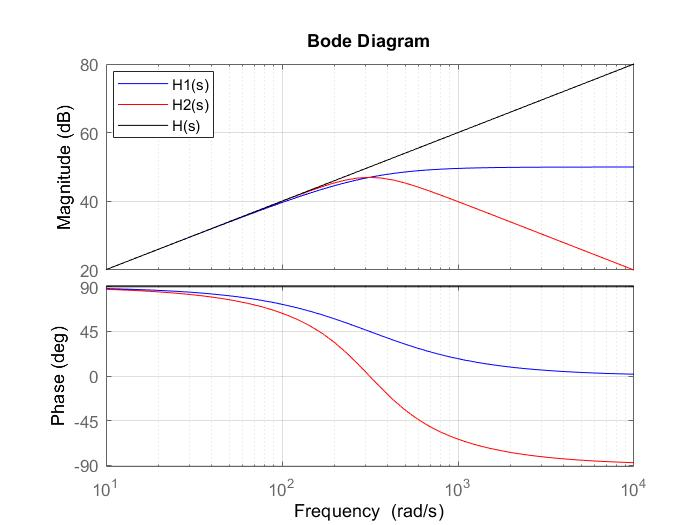
\includegraphics[scale=0.3]{BODEH.jpg}
\caption{Diagramma di Bode dei filtri}
\end{figure}

Dal diagramma di Bode si nota immediatamente come a basse frequenze entrambi i filtri approssimino bene il filtro ideale, mentre intorno alla frequenza di taglio $H_2(s)$ risulta essere migliore, ma solo per un breve intervallo. Dopo poco infatti $H_1(s)$ risulta essere evidentemente migliore.
Per quanto riguarda le fasi $H_1(s)$  si avvicina di più al modello ideale.

\subsection{Modellizzazione del motore}
Si modellizza il motore in corrente continua come segue: 
\begin{equation}
P(s)=\frac{1}{s}\frac{k_m}{T_m s + 1} \text{ \hspace{10 pt} con \hspace{10 pt}} k_m=5.2, T_m=0.03
\end{equation}

\subsection{Progettazione del controllore}
Si sviluppano due strategie di dimensionamento dei controllori:
\begin{itemize}
  \item Controllore P; 
  \item Controllore PI;
\end{itemize}

\subsubsection{Controllore P}
Si sfrutta il metodo del luogo delle radici per trovare il guadagno critico $K_P^*$ oltre il quale il sistema diventa instabile. Per avere un margine di stabilità si sceglie $K_P=K_P^* /4$. Viene qui riportato il luogo delle radici. 
\begin{figure}[H]
\centering
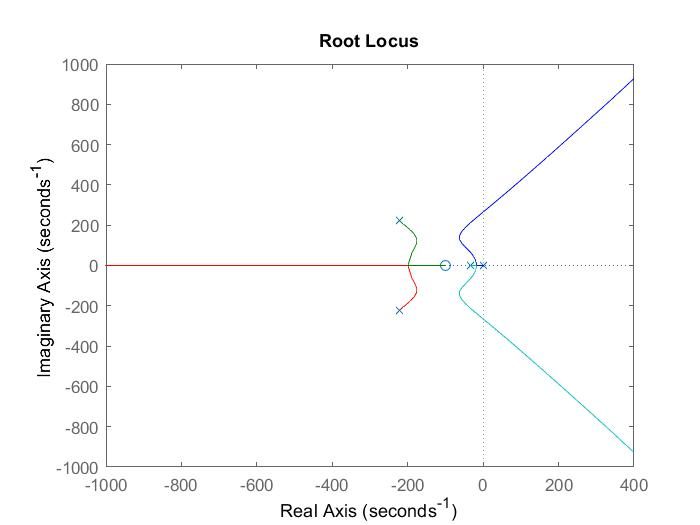
\includegraphics[scale=0.3]{rlocus.jpg}
\caption{Root Locus del sistema in catena chiusa}
\end{figure}
Dal luogo delle radici troviamo che $K_P^* = 2.9767 $.
\subsubsection{Controllore PI}
In questa strategia si sceglie un controllore PI il cui dimensionamento è dato: 
\begin{equation}
C(s)=K_P\frac{s + 100}{s}
\end{equation}

\section{Conclusioni}
\begin{figure}[H]
\centering
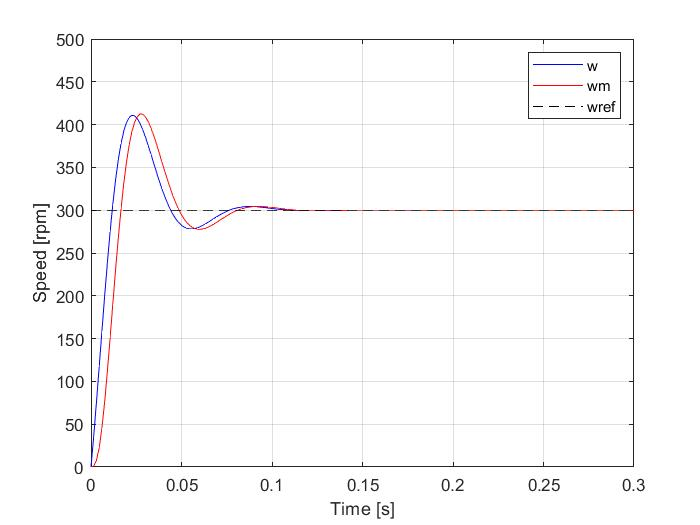
\includegraphics[scale=0.3]{pi.jpg}
\caption{Risposta al gradino con controllore PI}
\end{figure}
Dal grafico sopra riportato si evince che l'aggiunta di un polo nell'origine rende il sistema in grado di inseguire a regime senza errori un riferimento a gradino. Pertanto il controllore PI si rivela, per queste particolari specifiche, una scelta più adeguata.


\end{document}
